
% Template LaTeX - Iberoamerican Journal of Applied Computing (IJAC)
% ISSN 2237-4523

\documentclass[11pt,a4paper]{article}

\usepackage[utf8]{inputenc}
\usepackage[T1]{fontenc}
\usepackage[english]{babel}
\usepackage[a4paper,left=2.5cm,right=2.5cm,top=3.0cm,bottom=3.0cm]{geometry}
\usepackage{setspace}
\usepackage{ragged2e}
\usepackage{times}
\usepackage{xcolor}
\definecolor{ijacmaroon}{RGB}{115,20,40}

\usepackage{fancyhdr}
\pagestyle{fancy}
\fancyhf{}
\renewcommand{\headrulewidth}{0pt}
\renewcommand{\footrulewidth}{0pt}
\fancyhead[L]{\color{ijacmaroon}\bfseries\itshape\small Iberoamerican Journal of Applied Computing}
\fancyhead[R]{\color{ijacmaroon}\bfseries\itshape\small ISSN 2237-4523}
\fancyfoot[L]{\color{ijacmaroon}\bfseries\itshape V.XX, N\textsuperscript{o}.X, AAAA}
\fancyfoot[R]{\color{ijacmaroon}\bfseries\itshape Page \thepage}


\usepackage{tikz}
\usetikzlibrary{calc}
\AddToHook{shipout/background}{%
  
\begin{tikzpicture}[remember picture, overlay]
    \draw[ijacmaroon, line width=1.4pt]
      ($(current page.north west)+(2.5cm,-2.35cm)$) -- ($(current page.north east)+(-2.5cm,-2.35cm)$);
    \draw[ijacmaroon, line width=1.4pt]
      ($(current page.south west)+(2.5cm,2.3cm)$) -- ($(current page.south east)+(-2.5cm,2.3cm)$);
  \end{tikzpicture}%
}


\usepackage{titlesec}
\titleformat{\section}{\bfseries}{\thesection.}{0.5em}{}
\titleformat{\subsection}{\bfseries\itshape}{\thesubsection}{0.5em}{}
\titlespacing*{\section}{0pt}{1.5em}{0.8em}
\titlespacing*{\subsection}{0pt}{1.2em}{0.6em}


\usepackage{graphicx}
\usepackage{array}
\usepackage{caption}
\captionsetup[figure]{labelsep=endash,justification=centering,font=small}
\captionsetup[table]{labelsep=period,justification=centering,font=small,position=top}
\usepackage{booktabs}


\usepackage{hyperref}
\hypersetup{colorlinks=true,linkcolor=black,citecolor=black,urlcolor=blue}


\setlength{\parindent}{1.25cm}
\setlength{\parskip}{0pt}
\usepackage{indentfirst} 
\usepackage[alf,recuo=0cm,abnt-etal-text=it,bibjustif, abnt-emphasize = bf]{abntex2cite}
\begin{document}


\begin{center}
  {\large\bfseries Automated Detection of Coffee Leaf Diseases Using Convolutional Neural Networks and Transfer Learning}
  \vspace{0.8em}

  {\bfseries Camila R. Andrade$^1$, Bruno T. Almeida$^1$, Helena M. Duarte$^1$}
  \vspace{0.6em}

  $^1$Universidade Estadual de Ponta Grossa (UEPG) -- Ponta Grossa -- PR -- Brasil
  \vspace{0.3em}

  \texttt{candrade@uepg.br, balmeida@uepg.br, hduarte@uepg.br}
\end{center}

\vspace{1.2em}


\begin{quote}
\itshape
\noindent\textbf{Abstract.} Coffee leaf diseases are responsible for significant
yield losses in producing regions and are traditionally diagnosed through
visual inspection by agronomists, a process that is slow and dependent on
expert availability. This paper investigates the use of convolutional
neural networks and transfer learning to automatically identify three
common coffee leaf conditions -- rust, brown eye spot, and cercospora
leaf spot -- directly from smartphone images. A dataset of 2,450 leaf
images was collected in commercial plantations in the Ponta Grossa
region and expanded to 6,320 samples through data augmentation.
Four pretrained architectures (MobileNetV2, ResNet50, VGG16, and
EfficientNetB0) were fine-tuned on this dataset and compared in terms
of classification accuracy and inference time. The EfficientNetB0 model
achieved the best result, with an accuracy of 96.4\%, outperforming the
other architectures while requiring fewer computational resources.
These results indicate that lightweight transfer-learning models are a
viable option for on-device disease screening in precision agriculture
applications.

\vspace{0.6em}
\noindent\textbf{Keywords: machine learning, convolutional neural networks, transfer learning, plant disease detection}
\end{quote}

\vspace{1.0em}


\section{Introduction}

Coffee is one of the most economically important agricultural
commodities worldwide, and losses caused by foliar diseases can reach
a substantial fraction of a harvest when outbreaks are not identified
early \cite{antonelli2019}. Diagnosis is traditionally carried out by
agronomists through visual inspection of the leaves, a process that is
time-consuming, dependent on expert availability, and susceptible to
inconsistency between evaluators \cite{cope2012}.

Computer vision and deep learning have been increasingly explored as a
way to automate plant disease and species identification, allowing
non-experts to obtain a diagnosis directly from a smartphone photograph.
The contribution of this paper is twofold: a) a new image dataset of
coffee leaves affected by three common diseases, collected under field
conditions; b) a comparative evaluation of four convolutional neural
network architectures, using transfer learning, for the task of
automatic disease classification.

\section{Background}

Convolutional neural networks (CNNs) are hierarchical, multi-layer
feature extractors that have become the standard approach for image
classification tasks, including plant and leaf identification
\cite{lee2015deep}. When the number of labeled samples available for a
given task is limited, transfer learning is commonly used: a model
pretrained on a large, general-purpose dataset such as ImageNet is
fine-tuned on the smaller, task-specific dataset, allowing the
hierarchical features learned previously to be reused instead of
training a network from scratch \cite{zhuang2020}. This strategy has
been shown to reduce both training time and the amount of labeled data
required to reach a competitive accuracy.

\begin{figure}[htb]
  \centering
  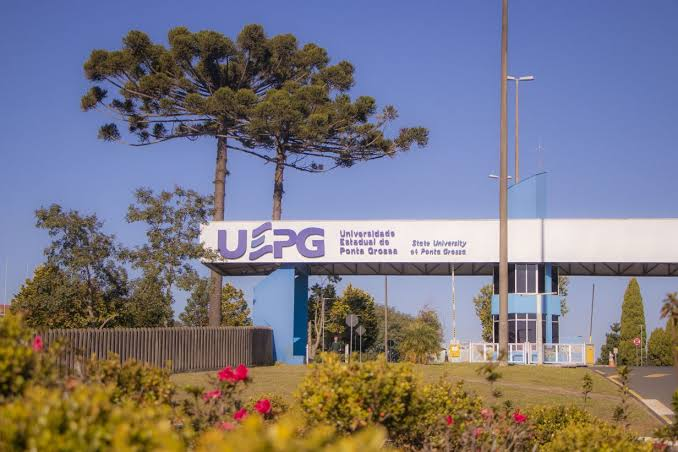
\includegraphics[width=0.7\linewidth]{figures/fig1}
  \caption{Overview of the transfer-learning pipeline: a pretrained convolutional base extracts features from the leaf image, and a new classification head is trained on the coffee leaf disease dataset (adapted from \cite{garcia2020})}
  \label{fig:exemplo}
\end{figure}

\section{Methods}

Leaf images were collected using smartphone cameras in commercial
coffee plantations located in the Ponta Grossa region, Paran\'a,
Brazil, between March and July 2024. Each image was labeled by an
agronomist into one of four classes: healthy, rust, brown eye spot, or
cercospora leaf spot. The initial set of 2,450 images was expanded to
6,320 samples using data augmentation techniques, including random
rotation, horizontal flipping, and brightness adjustment, in order to
reduce class imbalance and improve model generalization.

Four convolutional architectures pretrained on ImageNet --
MobileNetV2, ResNet50, VGG16, and EfficientNetB0 -- were used as
feature extractors. For each architecture, the original classification
head was replaced by a new fully connected layer trained on the coffee
leaf dataset, while the convolutional base was kept frozen during the
first training stage and partially unfrozen for fine-tuning in a
second stage. A total of 80\% of the images were used for training and
20\% for validation, with 60 training epochs for each model.

\section{Results}

Table \ref{tab:exemplo} summarizes the classification accuracy obtained
for each architecture on the validation set, together with the average
inference time per image measured on a mid-range mobile GPU.
EfficientNetB0 achieved the highest accuracy (96.4\%) while also
presenting the lowest inference time among the four models, making it
the most suitable candidate for deployment in a mobile screening
application. ResNet50 obtained a comparable accuracy (95.1\%) but at a
substantially higher inference cost, whereas MobileNetV2 offered the
best trade-off between accuracy and computational cost among the
remaining models.

\begin{table}[htb]
  \centering
  \caption{Validation accuracy and average inference time per image for each model.}
  \label{tab:exemplo}
  \begin{tabular}{|l|c|c|c|c|}
    \hline
    \textbf{Metric / Model} & \textbf{MobileNetV2} & \textbf{ResNet50} & \textbf{VGG16} & \textbf{EfficientNetB0} \\
    \hline
    Accuracy & 0.93 & 0.95 & 0.89 & 0.96 \\
    \hline
    Inference time (ms) & 42 & 118 & 96 & 38 \\
    \hline
  \end{tabular}
\end{table}

\section{Conclusion}

This paper presented a new coffee leaf disease image dataset and a
comparative evaluation of four convolutional neural network
architectures for automatic disease classification using transfer
learning. EfficientNetB0 obtained the best overall result, combining
the highest accuracy with the lowest inference time, which supports
its use in mobile, on-device screening applications for precision
agriculture. Future work includes expanding the dataset to additional
diseases and crop varieties, as well as evaluating the models under
field conditions with varying lighting and occlusion levels.

\bibliography{ijac-refs}

\end{document}
